%%%%%%%%%%%%%%%%%%%%%%
% \begin{itemize}
%     % \item Do not make the hypothesis that registers capture complementary info. We don't have evidence
%     % \item You need to consider OOD to understand the utility of registers
%     % \item Darcet etal wanted to isolate high-norm tokens through registers. In that process it aggregates gloabl information. We are proposing that it can be viewed as secondary information. 
%     % \item From ID standpoint, they might seem redundant, we need to consider OOD to determine the utility of registers
%     % \item Finding, we find that registers lead to rich feature representation. 
%     % \item High-norm tokens do not pose a problem for classification. It is only for object discovery. From that standpoint with or without registers should not matter. (which is not true)
%     % \item We study as a secondary feature representation. Given that it is  low degrees of freedom, it doesnot fully represent. Motivation figure. Only CLS , only register
%     % \item However, feature richness, inherent performance they can lead to imporvec generalization. 
%     % \item In this paper, we want to explore if these secondary representations with primary from CLS do they lead to improved gen. Surprisingly. we find that ..
%     % \item We want to emphasize that ..
% \end{itemize}
%%%%%%%%%%%%%%%%%%%%%%


%%%%%%%%%%%%%%%%%%%%%%
% Vision Transformers (ViTs)~\cite{dosovitskiy2021an}, which adapt the transformer architecture from natural language processing~\cite{vaswani2017attention}, have demonstrated exceptional performance across a range of vision tasks including classification and object detection~\cite{touvron2022deit, dettmers2022gptint, peebles2023scalable}. At a high level, ViTs process images by dividing them into fixed-size patches, each treated as a token, with a special \texttt{[CLS]} token appended to aggregate information across tokens for downstream tasks.

% In a recent work on the behavior of large scale ViTs by Darcet \textit{et al.}~\cite{darcet2024vision}, it was observed that patch tokens associated with low-informative regions (e.g., background) tend to have notably higher $\ell_2$ norm values compared to other tokens. While this tendency does not impact their utility in image-level prediction tasks, it increases the risk of compromising the performance in dense prediction tasks (e.g., object discovery). To circumvent this behavior, the authors explored the use of ``registers", which are additional tokens appended to the input sequence during training. 


% Interestingly, these register tokens not only isolate the behavior of the high norm tokens but also were observed to capture global information when a linear classifier was trained with register token embeddings extracted for the in-distribution data. While the utility of registers in enabling smoother attention maps and thus improved performance in object discovery has been well studied, their utility in solving downstream image classification tasks are yet to be uncovered, which is the focus of this paper. To achieve this objective, and to to completely understand the utility of registers we also need to consider their OOD generalization performance. 
% As results from Figure~\ref{} show that registers due to their low degrees of freedom by themselves do not capture all the information required to achieve robust features.

% Consequently, in this paper, we investigate the utility of registers as auxiliary features supplementing the CLS token embeddings to obtain rich features which enable robust adaptation, similar to findings from Zhang et al where seemingly redundant features  w.r.t to ID performance can lead to significant gains in OOD settings. 

% To that end, we train an LC by combining the CLS token and aggregated register embeddings (avg pooled) and we make a striking finding that while our proposed approach maintains the ID performance obtained by using only CLS, it achieves significantly superior performance on two critical tasks, namely,  out-of-distribution (OOD) generalization and anomaly rejection two major components in understanding the robustness of the resulting features. Our extensive experiments, spanning multiple ViT backbones, demonstrate that our method consistently outperforms baseline approaches by \textbf{2-3\%} increase in top-1 accuracy for OOD generalization and an average reduction of an average of \textbf{4.2\%} in the false positive rate for anomaly detection. 
% These findings thus support our hypothesis that the registers when combined with CLS token can produce robust feature representations. Importantly, these gains are obtained with a negligible computational overhead.

% In summary, our contributions are as follows:
% \begin{itemize}
%     \item We develop a novel method that leverages the register token embeddings as auxiliary features for building robust adaptation protocols.
%     \item Through extensive experiments, we demonstrate consistent improvements in OOD generalization and anomaly detection across multiple ViT architectures.
%     \item We show that our method achieves these gains with negligible computational overhead during training or inference, offering efficient solution.
% \end{itemize}
%%%%%%%%%%%%%%%%%%%%%%


\section{Introduction}


\begin{figure}[t]
    \centering
    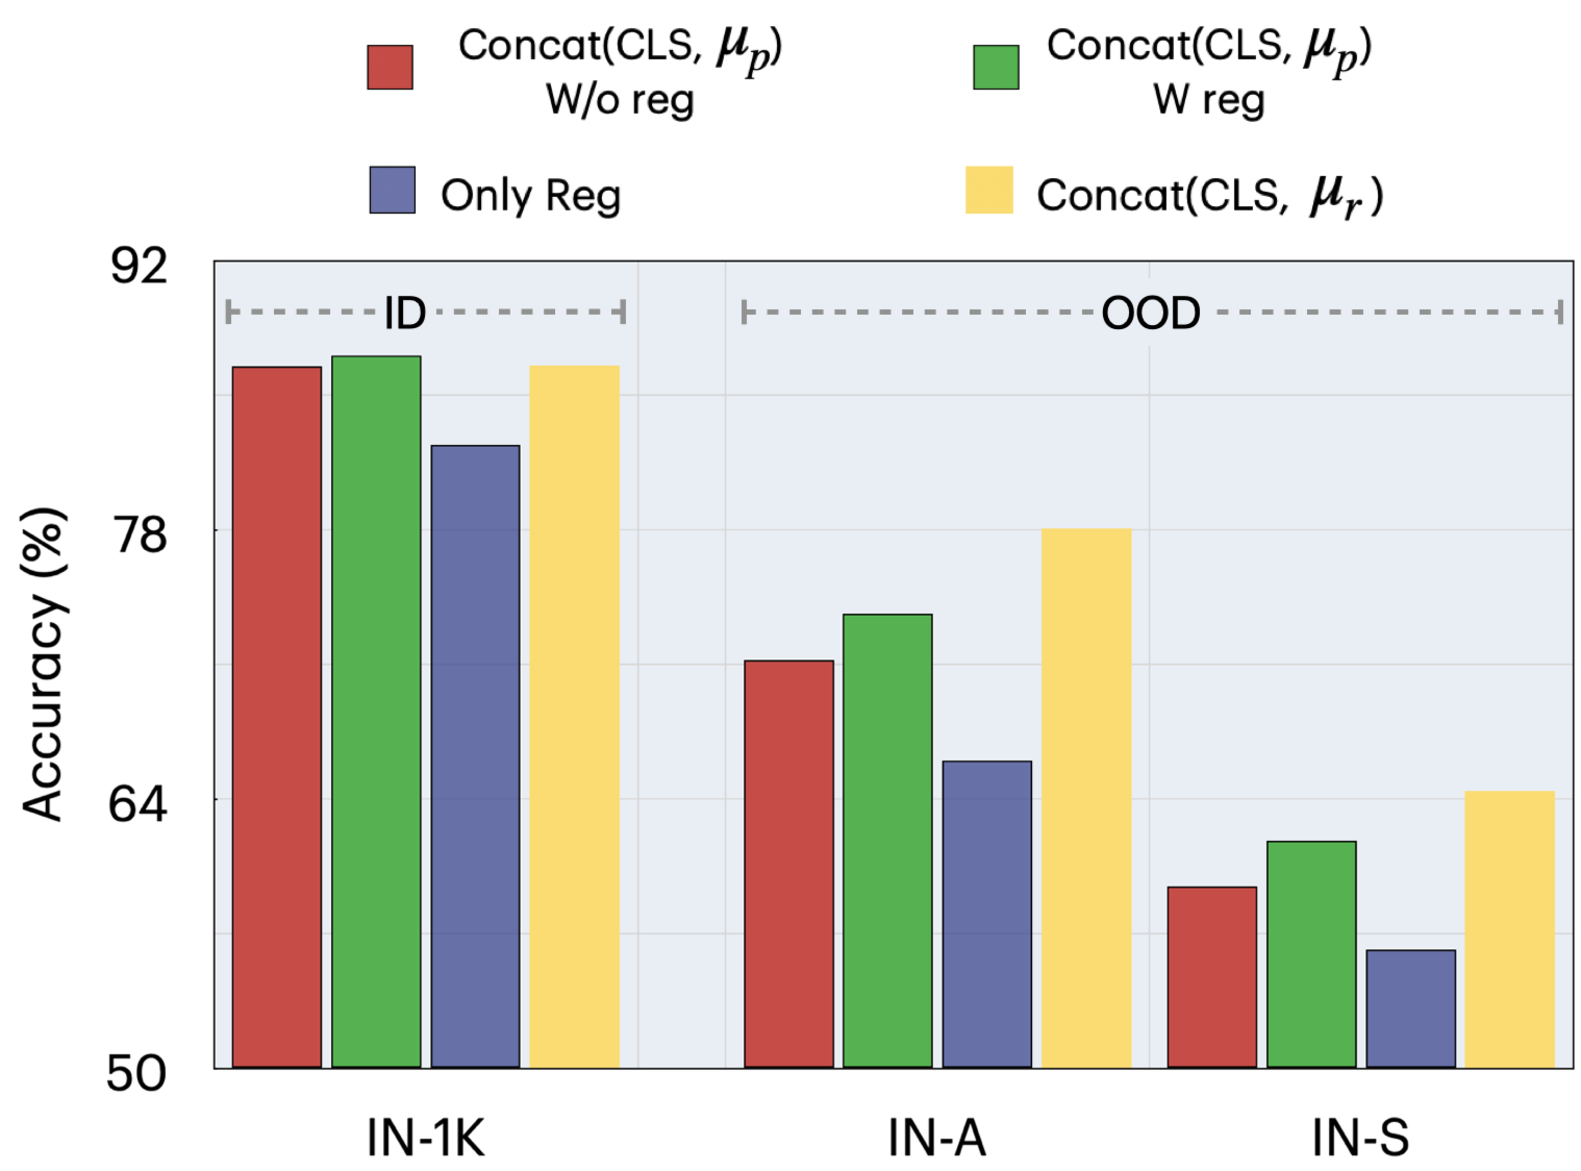
\includegraphics[width=1\linewidth]{figures/teaser_fig.pdf}
    \caption{\textbf{Impact of token embedding choices on linear probing on frozen Dino-V2 ViT-G backbones. } Each color indicates the token embeddings chosen for optimizing a linear classifier on ImageNet (IN)-1K along with the protocol adopted for pre-training the backbone (w/o registers or w registers). Here, \texttt{[CLS]} represents the classification token, $\mu_P$ and $\mu_R$ represents the mean patch and register token embeddings respectively. While it is common to utilize \texttt{[CLS]} and $\mu_P$ to train the classifier, we obtain improved generalization if the backbone is trained with registers (red vs green). Training a classifier naively with register tokens results in drop in generalization. However, our approach (yellow) maintains ID accuracy while providing substantial gains in OOD (ImageNet-Adversarial, ImageNet-Sketch) accuracies.}
    \label{fig:motivation}
\end{figure}

Vision Transformers (ViTs)~\cite{dosovitskiy2021an}, which adapt the transformer architecture from natural language processing~\cite{vaswani2017attention}, have demonstrated exceptional performance across a range of vision tasks including classification and object detection~\cite{touvron2022deit, dettmers2022gptint, peebles2023scalable}. At a high level, ViTs process images by dividing them into fixed-size patches, each treated as a token, with a special \texttt{[CLS]} token appended to aggregate information across tokens for downstream tasks.

In a recent study on the behavior of large scale ViTs,  Darcet \textit{et al.}~\cite{darcet2024vision} observed that patch tokens associated with low-informative regions (e.g., background) tend to have significantly higher $\ell_2$ norm values compared to other tokens. While this tendency does not impact their utility in image-level prediction tasks, it increases the risk of compromising the performance in dense prediction tasks (e.g., object discovery). To circumvent this behavior, the authors explored the use of ``registers", which are additional tokens appended to the input sequence during training. Interestingly, these registers were found not only to isolate the behavior of the high norm patch tokens but also contain global image-level information. This was validated when a linear classifier was trained on register token embeddings extracted from in-distribution (ID) data, demonstrating enhanced classification performance.

While the utility of registers in achieving improving object discovery has been well studied, their efficacy in downstream tasks such as classification remains under explored, which is the primary focus of our paper. To thoroughly assess the role of registers in these tasks, it is critical to evaluate their generalization capabilities under a variety of out-of-distribution (OOD) scenarios.  As shown in Figure~\ref{fig:motivation}, naively training a linear classifier with register token embeddings results in a non-trivial drop in generalization performance on OOD datasets implying that the registers by themselves do not capture all the information required to achieve robustness. 



Consequently, in this paper, we examine the utility of  register token embeddings, which are shown to contain global image-level information, as auxiliary features that supplement the \texttt{[CLS]} token embedding. We believe that such a combination will yield in enriched representations for robust adaptation. This hypothesis aligns with the findings of Zhang \textit{et al.}~\cite{zhang2023learning}, where seemingly redundant features with respect to in-distribution data provided significant benefits in OOD scenarios when combined together.

\begin{figure*}[!t]
    \centering
    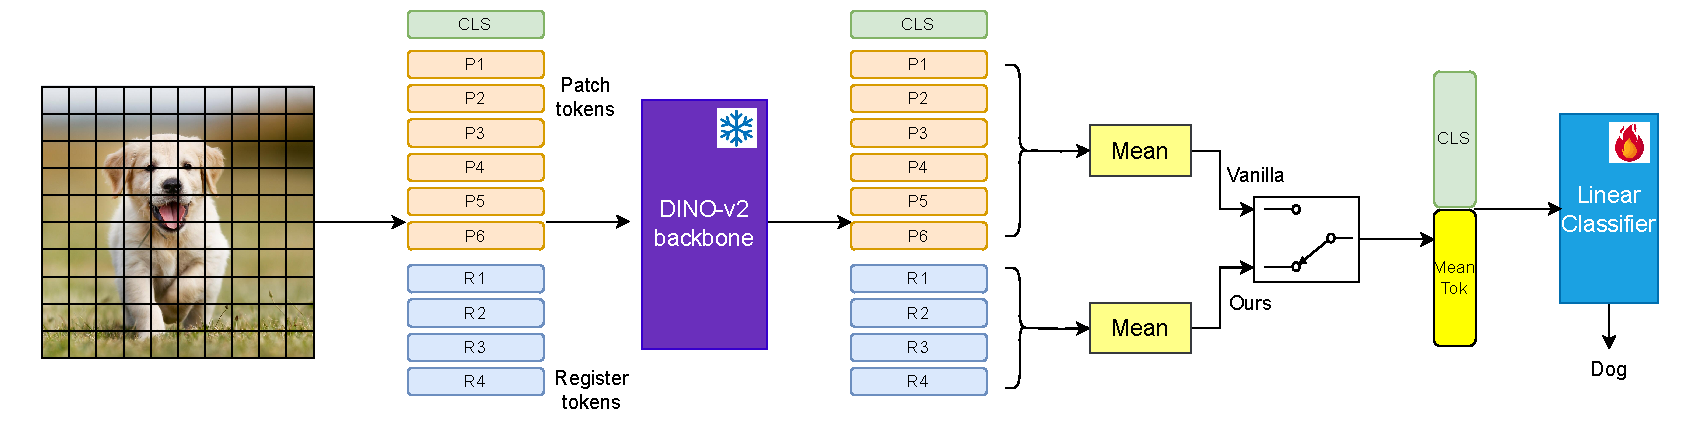
\includegraphics[width=\linewidth]{figures/method.pdf}
    \caption{\textbf{Overview of our proposed method}: For large-scale vision transformer backbones (e.g., DINO-v2) pre-trained with ``registers", we find that concatenating registers (Mean (R$_1$, R$_2$, R$_3$, R$_4$) along with \texttt{[CLS]} is critical for obtaining rich features that enable robust adaptation. In particular, we train a linear classifier on these concatenated features and observe improved generalization and anomaly rejection capabilities.}
    \label{fig:method}
\end{figure*}

To that end, we train a linear classifier by combining the representations from the \texttt{[CLS]} token with the average-pooled register token embeddings $\mu_R$. We compare our approach with the standard practice of combining \texttt{[CLS]} token with average-pooled patch tokens $\mu_P$ \cite{oquab2023dinov2}. Strikingly, our method significantly improves both OOD generalization, while maintaining ID performance, as shown in Fig \ref{fig:motivation}. Moreover, our approach also boosts anomaly rejection performance, compared to baselines. Our comprehensive experiments across multiple ViT backbones reveal a consistent improvement of \textbf{2-4\%} in top-1 accuracy for OOD generalization and an average reduction of \textbf{2-3\%} in the false positive rate for anomaly detection. These findings support our hypothesis that the concatenation of registers with \texttt{[CLS]} yields more robust feature representations. Importantly, these gains are obtained without incurring any additional computational overhead.

In summary, our contributions are as follows:
\begin{itemize}
    \item We develop a novel method that leverages the register token embeddings as auxiliary features for building robust adaptation protocols.
    \item Through extensive experiments, we demonstrate consistent improvements in OOD generalization and anomaly detection across multiple ViT architectures.
    \item Our method achieves these gains with negligible computational overhead during training or inference, offering an efficient solution.
\end{itemize}